% Sustainable Raw Material Benchmarking — paper
% Build: pdflatex sustainable_raw_material_benchmarking.tex  (run twice for the contents)
\documentclass[10pt,twocolumn,a4paper]{article}

\usepackage[T1]{fontenc}
\usepackage[utf8]{inputenc}
\usepackage{textcomp}
\usepackage[margin=2.0cm,columnsep=0.72cm]{geometry}
\usepackage{booktabs}
\usepackage{graphicx}
\usepackage{amsmath}
\usepackage{amssymb}
\usepackage{rotating}
\usepackage{xcolor}
\usepackage{array}
\usepackage{enumitem}
\usepackage{caption}
\usepackage{titlesec}
\usepackage{ragged2e}
\usepackage[hidelinks]{hyperref}

\definecolor{ink}{HTML}{14181B}
\definecolor{ink2}{HTML}{3D474D}
\definecolor{ink3}{HTML}{6E7B82}
\definecolor{pblue}{HTML}{2E5A87}
\definecolor{pgreen}{HTML}{3E8F63}
\definecolor{pred}{HTML}{B3372C}
\definecolor{pamber}{HTML}{B57C15}

\captionsetup{font=small,labelfont=bf,labelsep=period,justification=justified}
\captionsetup[table]{skip=4pt}
\setlist{nosep,leftmargin=1.2em}
\titlespacing*{\section}{0pt}{2.0ex plus .3ex}{0.9ex}
\titlespacing*{\subsection}{0pt}{1.4ex plus .2ex}{0.6ex}
\renewcommand{\arraystretch}{1.12}
% float placement: without these, late figures are deferred past the
% bibliography and land on near-empty pages
\renewcommand{\topfraction}{0.92}
\renewcommand{\bottomfraction}{0.70}
\renewcommand{\textfraction}{0.06}
\renewcommand{\floatpagefraction}{0.70}
\setcounter{topnumber}{3}
\setcounter{totalnumber}{5}

\newcommand{\co}{CO\textsubscript{2}e}
\newcommand{\eur}[1]{EUR~#1}
\newcommand{\dimhead}[1]{\textbf{#1}}
\newcommand{\ev}[1]{{\footnotesize\textsc{#1}}}
\newcommand{\synth}{\textit{Synthetic demonstration data.}}

\title{\vspace{-1.4em}\Large\bfseries Benchmarking Sustainable Raw Material
Alternatives Without a Sustainability Score\\[0.35em]
\large\mdseries Eligibility, comparability, evidence and trade-off: a decision method
demonstrated on a synthetic chemical-procurement dataset and an analytics prototype}
\author{Csaba Bakay}
\date{August 2026}

\begin{document}
\maketitle

\begin{abstract}
\noindent
Procurement organisations are increasingly asked to compare raw-material
alternatives on cost and carbon at the same time. The difficulty is no longer
calculating a product carbon footprint; it is turning one into something a
sourcing decision can use. The comparison fails in three specific ways: options are compared that cannot actually be bought, numbers are
compared that were never calculated on the same basis, and dimensions are merged
that should have stayed apart. None of these failures is solved by a better
score.

This paper develops a decision method organised as a sequence --- establish
\emph{eligibility}, then establish \emph{comparability}, then show the
\emph{trade-off}, with evidence assessed before the trade-off is put to a named
decision owner. Ten success dimensions give the decision context a structured
view, each made assessable through measurement indicators and read against a
benchmark rather than combined into one figure. The method is supported by a
four-role convention that separates gates from
performance, evidence and context; by an operationalisation of the six
comparability conditions of the GHG~Protocol \emph{Product Standard},
Appendix~A~\S A.1; and by an evidence model that keeps provenance, data quality,
verification and uncertainty outside the performance number.

The method is demonstrated on a synthetic dataset of 25 material alternatives
across five independent benchmark cases, carrying deliberately embedded
data-quality defects, harmonised through a deterministic pipeline into an audited
semantic layer of 21 measures and displayed through a working analytics
prototype. Four findings are named: the portfolio total is overstated
approximately fivefold when mutually exclusive scenarios are summed; the two
options with the strongest cost and carbon position in one case are both
technically blocked; the strongest carbon result in another case rests on a 2019
industry-average factor; and one material has no carbon figure at all and is
never assigned one.

The paper states plainly what the demonstrator does \emph{not} establish. No
\S A.1 comparability condition is fully satisfied by it today, and the eight
fields that would close the gap are named. All data is synthetic and labelled as
such. No sustainability score, weighting or cross-case ranking is produced at any
point.
\end{abstract}

{\small\tableofcontents}
\vspace{0.6em}

% ═══════════════════════════════════════════════════════════════════════
\section{Introduction}

Raw-material sourcing decisions have acquired a second objective. Where a
category manager once had to reconcile price, quality and security of supply, the
same decision is now also expected to deliver a carbon reduction, and to
withstand questioning about water, circularity, hazardous substances and supply
concentration. A common organisational response is to add columns to a
supplier scorecard.

That response misdiagnoses the problem. Adding columns assumes the difficulty is
a shortage of dimensions. It is not. The difficulty is that the dimensions behave
differently in a decision, that the numbers placed in those columns are frequently
not comparable with one another, and that a large share of the cells are empty in
a way that a scorecard conceals rather than reports.

This paper takes the opposite route. Instead of enriching a score, it removes the
score and replaces it with a sequence:

\begin{center}\small
\textsc{eligibility} $\rightarrow$ \textsc{comparability} $\rightarrow$ \textsc{evidence}\\
$\rightarrow$ \textsc{trade-off} $\rightarrow$ \textsc{decision and governance}
\end{center}

\noindent An alternative must first be shown to be \emph{eligible} --- legally and
technically capable of being bought. Its figures must then be shown to be
\emph{comparable} with the incumbent's, and the \emph{evidence} behind those
figures must be assessed rather than assumed. Only then is the remaining
\emph{trade-off} put in front of a named decision owner, who records the decision
and what was given up. Each step has a failure mode that is invisible if the steps
are collapsed.

The argument is developed on a synthetic demonstrator rather than on industrial
data. This is a deliberate constraint and it has a cost, discussed in
Section~\ref{sec:limits}. It also has a benefit: because the dataset was
authored, its data-quality defects are known exactly, and the method can be shown
handling them rather than asserted to handle them.

\paragraph{Contributions.} The main contributions are:
\begin{enumerate}[label=\arabic*.]
  \item a decision sequence that makes each failure mode visible before the next
        one is judged;
  \item ten success dimensions, each made assessable through measurement
        indicators and read against a benchmark rather than aggregated;
  \item a four-role convention --- gate, performance, evidence, context ---
        presented explicitly as a project synthesis rather than a validated
        framework;
  \item an operationalisation of the six \S A.1 comparability conditions as a
        three-state verdict usable inside a sourcing decision;
  \item an evidence model separating provenance, data quality, verification and
        uncertainty from the performance number, with missing values preserved as
        missing at four independent layers;
  \item a reproducible synthetic demonstrator, and an explicit statement of what
        it does not establish together with the fields that would close the gap.
\end{enumerate}

% ═══════════════════════════════════════════════════════════════════════
\section{Background and related work}

\subsection{What the standards settle}

The methodological base for product-level carbon accounting is mature. The
GHG~Protocol \emph{Product Life Cycle Accounting and Reporting Standard}
\cite{p1} defines how a product carbon footprint (PCF) is calculated, and
ISO~14040/14044 with the associated pedigree guidance \cite{a2} define what data
quality means in a life-cycle inventory. For the chemical sector, the
\emph{Together for Sustainability} PCF guideline \cite{b1} and the cross-sector
PACT methodology \cite{p3,b2} specify how a supplier-declared footprint should be
produced and exchanged; the Catena-X rulebook \cite{b3} does the same for
automotive value chains. ISO~20400 \cite{a1} places sustainability criteria
alongside price and quality inside a single procurement evaluation rather than in
a parallel process.

Beyond climate, methods also exist and are frequently assumed not to.
ISO~14046 \cite{v3} defines a product water footprint including consumption and
degradation, with mandatory attention to local hydrological conditions. The EU
Product Environmental Footprint, recommended for use by Commission Recommendation
(EU) 2021/2279 \cite{v4}, covers sixteen impact categories including toxicity,
land use and resource depletion, operationalised per product group through
category rules.

The regulatory frame adds duties rather than decision rules: ESRS topical
standards E1--E5 \cite{a4}, the Critical Raw Materials Act \cite{a3}, the Carbon
Border Adjustment Mechanism \cite{a7}, the Ecodesign for Sustainable Products
Regulation \cite{a6}, and corporate sustainability due diligence as amended by
Directive (EU) 2026/470 \cite{p5,v1}. REACH \cite{v2,p4} defines specific
prohibitions and specific information duties, which --- as Section~\ref{sec:roles}
shows --- are frequently confused with one another.

\subsection{What the standards do not settle}

Three gaps matter for a sourcing decision.

First, the carbon standard limits itself explicitly. \S1.7 of \cite{p1} sets out
that a climate-only inventory can miss trade-offs and co-benefits across other
environmental impacts, and directs that its results \textbf{not be treated as a
statement of a product's overall environmental performance}.\footnote{The
standard names ecosystem degradation, resource depletion, ozone depletion and
negative human health impacts among the categories at risk \cite{p1}.}

Second, the same standard states that it does not, by itself, support the
comparison a buyer wants to make. Appendix~A distinguishes the intended
applications; performance tracking is supported as published, while consumer and
business purchasing decisions require additional programme specifications or
product-specific guidance. Section~\ref{sec:comparability} makes this operational.

Third, the literature on decision method is thin where it matters most. Material
selection under constraints is well established \cite{c6,c5}, and life-cycle data
quality has an established vocabulary \cite{a2,c7}, but neither tells a category
manager what to do when the best-performing candidate is not approved, or when the
best carbon figure has the weakest provenance. That gap is where this paper sits.

% ═══════════════════════════════════════════════════════════════════════
\section{Success dimensions and measurement indicators}

A sourcing decision is easier to argue when the dimensions it turns on are named
before the numbers arrive. Success dimensions provide a structured view of the
decision context. Suitable measurement indicators make each dimension assessable
against a relevant benchmark. The reference point may be a target level, a peer
profile or --- as in the demonstrator from Section~\ref{sec:problem} onward ---
the incumbent. Figure~\ref{fig:profile} illustrates how such a
multidimensional benchmark profile can be visualised without aggregating the
dimensions into a single score.

\begin{center}\small
success dimensions $\rightarrow$ measurement indicators\\
$\rightarrow$ benchmark comparison $\rightarrow$ decision support
\end{center}

Table~\ref{tab:dimensions} lists ten dimensions that recur in raw-material
sourcing, with examples of the indicators that make them assessable. Which
dimensions are relevant, and which indicators are suitable, depends on the
material, the application and the decision context.

\paragraph{Reading the profile.} The value of the profile is in its shape. A
profile that meets the benchmark on eight dimensions and falls two levels short
on one is a different decision from a profile that is uniformly one level short,
even though a single combined figure would treat them alike. Keeping the
dimensions apart is what preserves that difference.

\begin{figure*}[t]
  \centering
  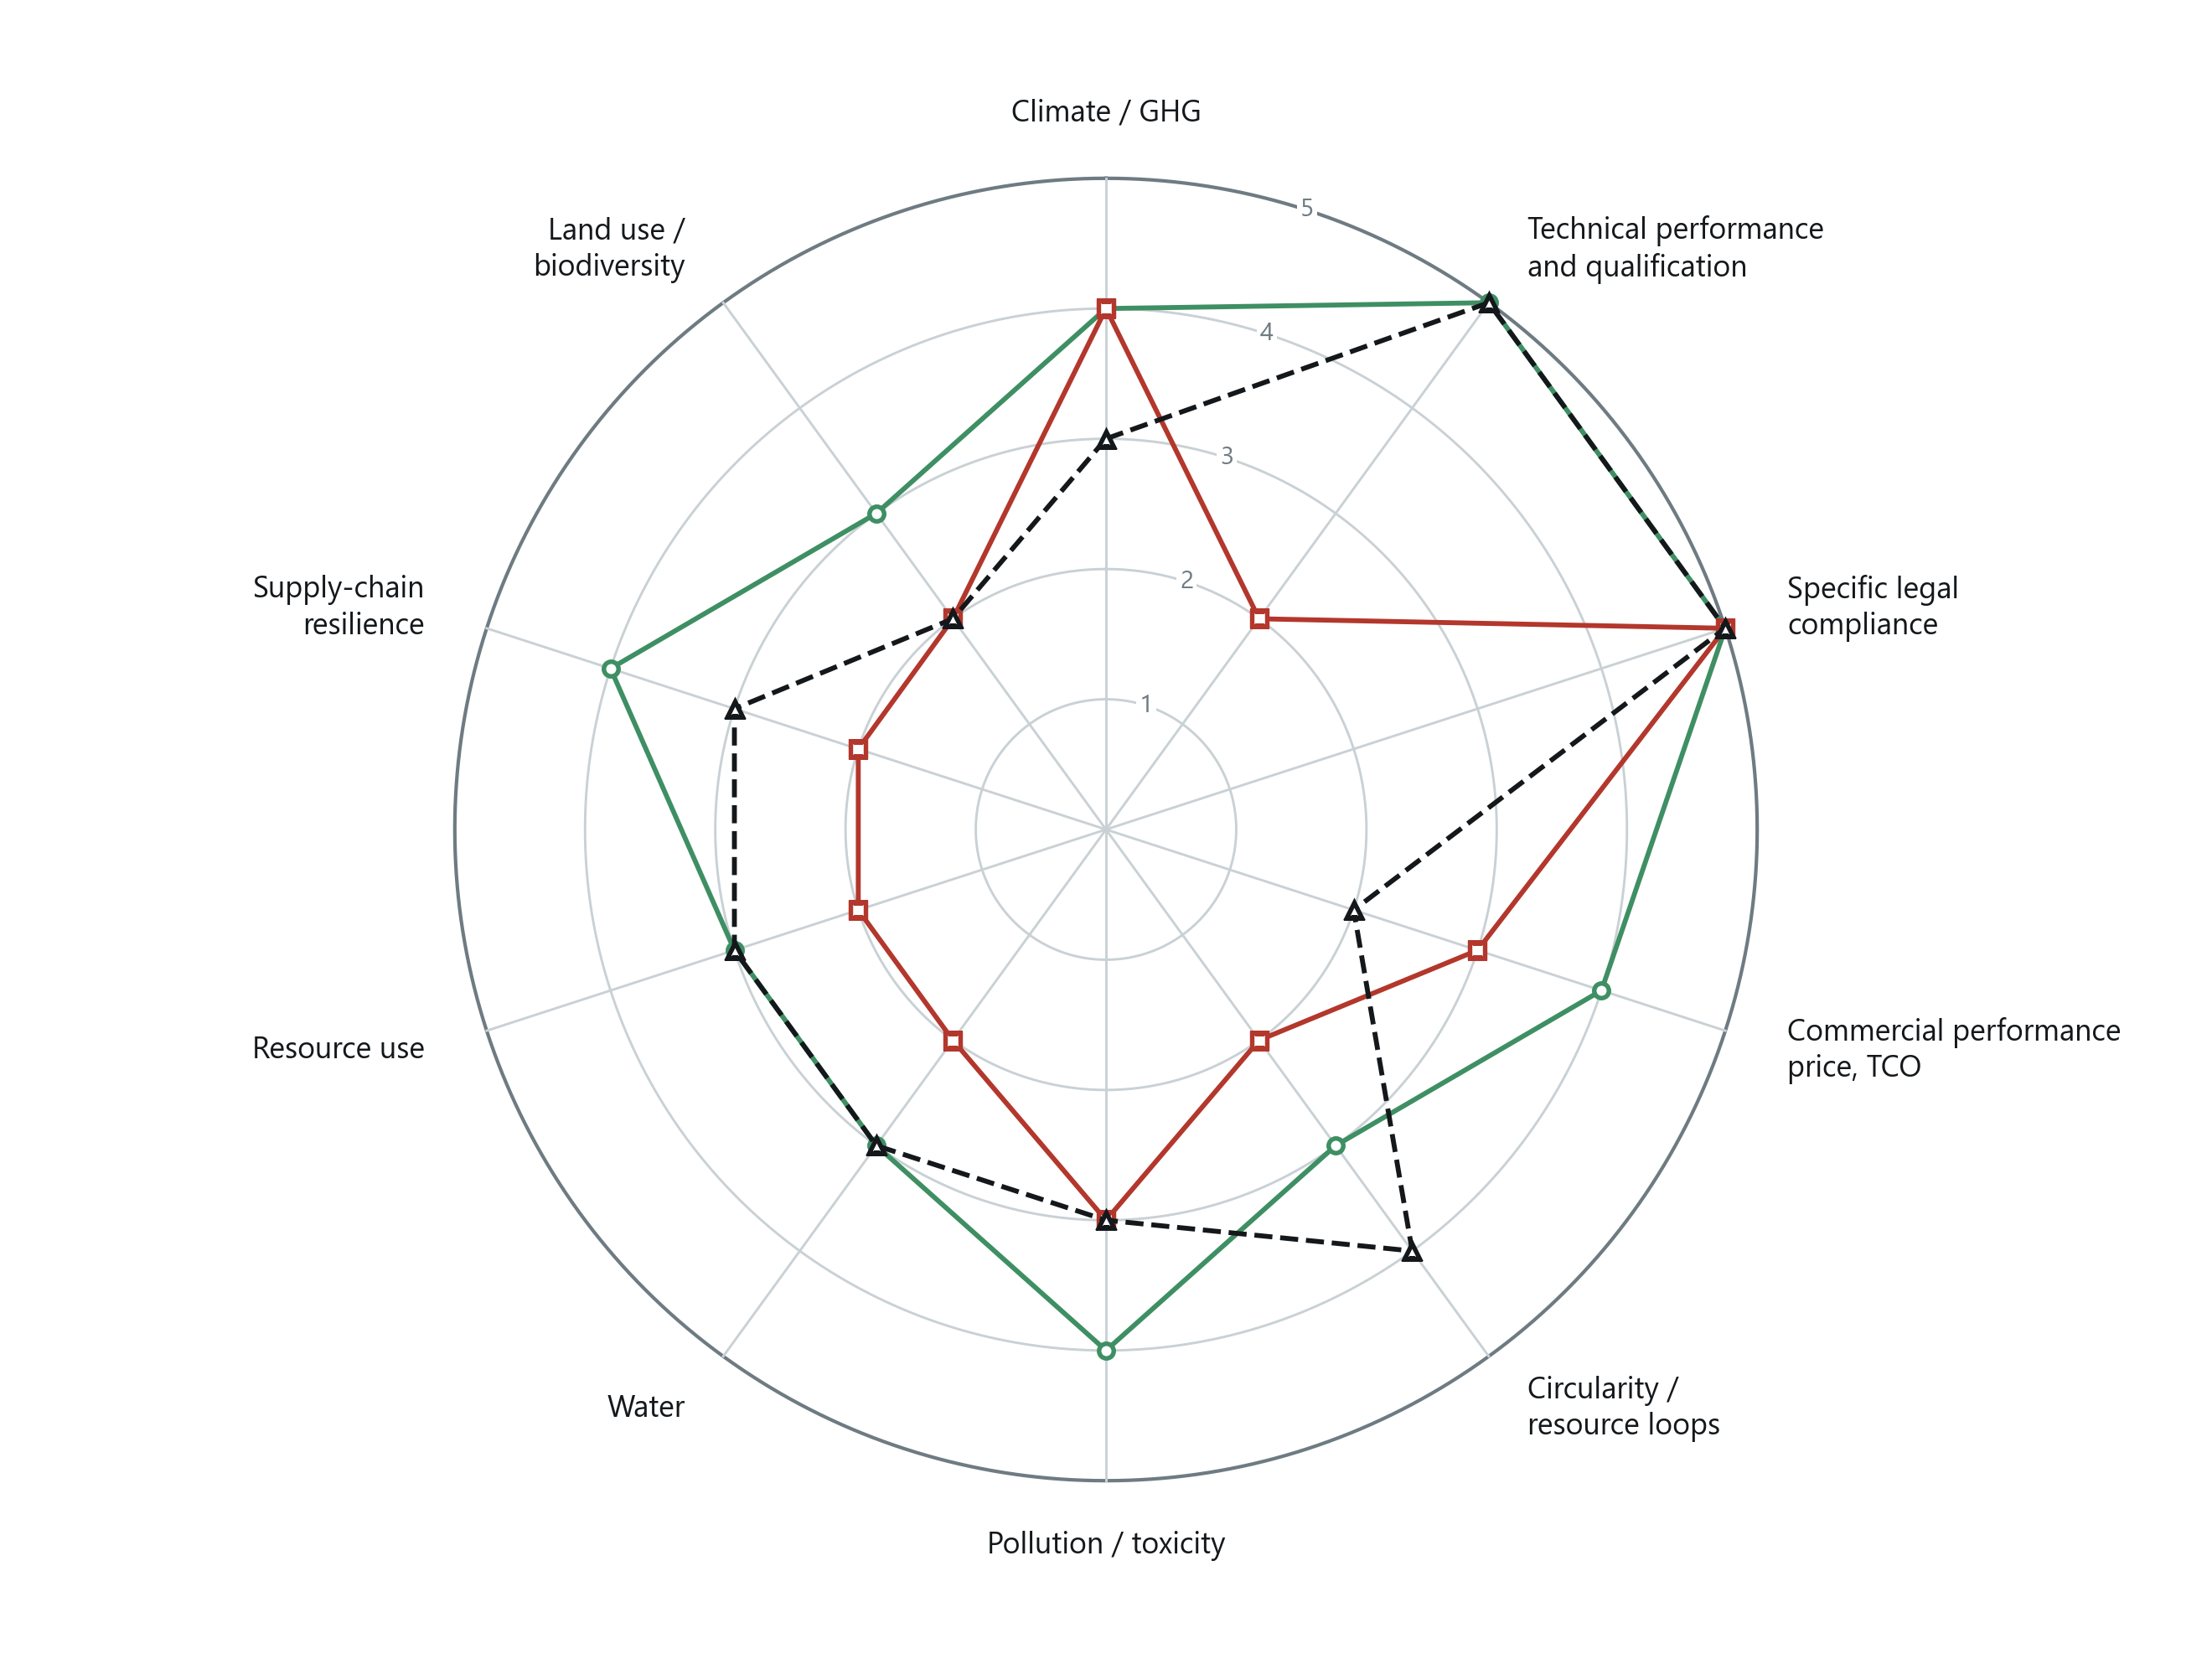
\includegraphics[width=0.80\textwidth]{figures/fig01_benchmark_profile.png}
  \caption{A multidimensional benchmark profile. Ten success dimensions on a
  common five-level scale, each read against a benchmark rather than combined
  with the others. Green marks the benchmark or target level, red the observed
  profile, black a second profile for comparison. \textbf{The values shown are
  illustrative examples, not empirical assessments.} The dimensions stay
  separate: no weighting is applied, no total is formed and no ranking is
  derived.}
  \label{fig:profile}
\end{figure*}

\begin{table*}[t]
  \caption{Ten success dimensions that recur in raw-material sourcing, with
  examples of the measurement indicators that make each one assessable. The class
  column records how far a dimension enters this project's scope, not its
  decision role: \textsc{a}~core, \textsc{b}~context-dependent,
  \textsc{c}~acts as a gate condition, \textsc{d}~relevant to the wider picture
  but outside this prototype. Which dimensions are relevant, and which indicators are suitable,
  depends on the material, the application and the decision context.}
  \label{tab:dimensions}
  \small
  \begin{tabular}{@{}p{0.030\textwidth}p{0.235\textwidth}p{0.035\textwidth}p{0.60\textwidth}@{}}
    \toprule
    & \dimhead{Success dimension} & \dimhead{Class} & \dimhead{Example measurement indicators} \\
    \midrule
    1 & Climate / GHG & \textsc{a} & PCF in kg \co{} per kg; \co{} delta vs incumbent; PCF coverage; evidence attributes \\
    2 & Technical performance and qualification & \textsc{c} & Approval status; equivalence against the technical specification; qualification stage \\
    3 & Specific legal compliance & \textsc{c} & Authorisation or restriction status for the specific use; company policy thresholds \\
    4 & Commercial performance --- price, TCO & \textsc{a} & Price per kg; annual spend; cost delta vs incumbent; qualification and switching cost \\
    5 & Circularity / resource loops & \textsc{b} & Recycled and renewable content; chain-of-custody model; retention of value \\
    6 & Pollution / toxicity & \textsc{b} & PEF toxicity categories; substance profile for the actual use and exposure \\
    7 & Water & \textsc{b} & ISO 14046 water footprint; basin-level water stress at the production site \\
    8 & Resource use & \textsc{b} & PEF resource-use categories; feedstock intensity \\
    9 & Supply-chain resilience & \textsc{b} & Awarded-volume concentration; dual-source status; lead time and recovery time \\
    10 & Land use / biodiversity & \textsc{d} & Land-occupation and transformation by origin; feedstock-specific pressure \\
    \bottomrule
  \end{tabular}
\end{table*}

% ═══════════════════════════════════════════════════════════════════════
\section{Problem formulation}
\label{sec:problem}

\begin{figure*}[t]
  \centering
  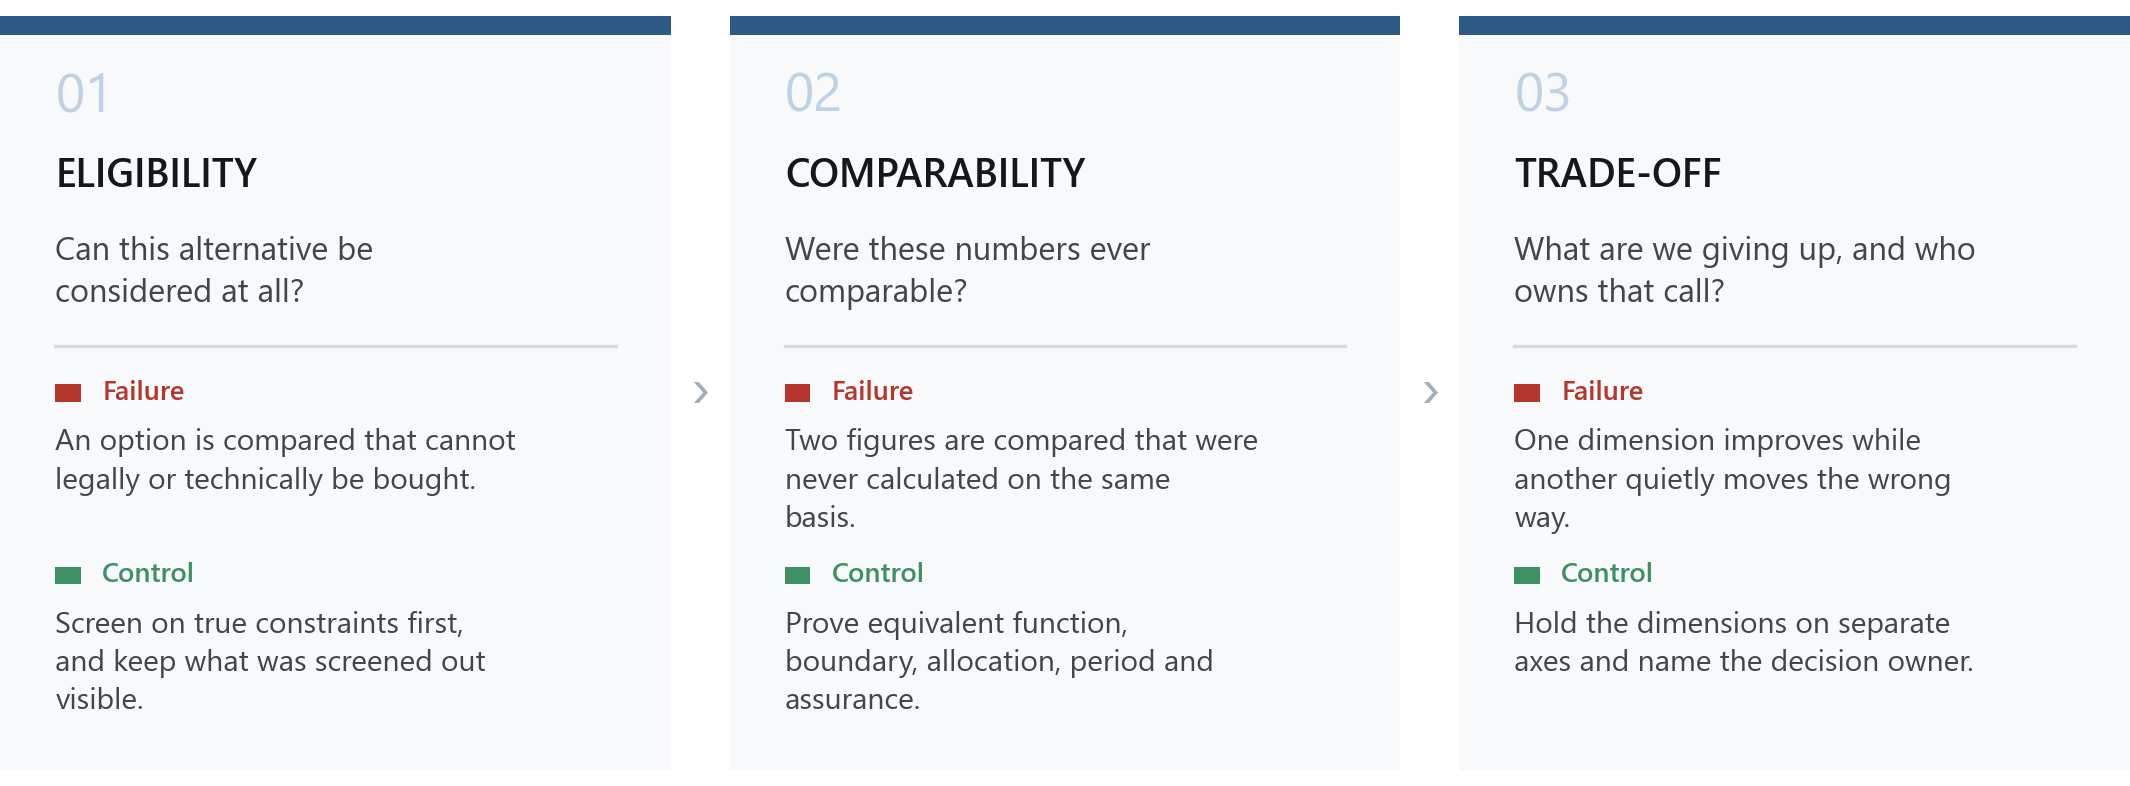
\includegraphics[width=\textwidth]{figures/fig02_decision_sequence.png}
  \caption{The three failure modes and the sequence that answers them. Each stage
  states the question it settles, the failure that occurs when it is skipped, and
  the control that prevents it. The sequence is not a workflow diagram: it is an
  ordering constraint, and its value is that a later stage may not repair an
  earlier one.}
  \label{fig:sequence}
\end{figure*}

\subsection{Comparison cases and the incumbent baseline}

A benchmark exercise is organised into \emph{cases}. A case $c$ is one purchased
material need, containing exactly one incumbent $b(c)$ --- the material currently
bought --- and a set of candidate alternatives. Cases are independent: an
alternative in one case is not substitutable for an alternative in another, so no
statement is made across cases.

Within a case, performance is expressed relative to the incumbent. For an
alternative $i$ in case $c$, with annual spend $s_i$ and annual emissions $g_i$,

\begin{equation}
  \Delta^{\text{cost}}_i = \frac{s_i - s_{b(c)}}{s_{b(c)}},
  \qquad
  \Delta^{\co}_i = \frac{g_i - g_{b(c)}}{g_{b(c)}}.
  \label{eq:delta}
\end{equation}

Two properties of Equation~\eqref{eq:delta} carry the method. First, both deltas
are computed from absolute quantities, not from stored percentages, so a rounded
column can never enter a decision. Second, $\Delta^{\co}_i$ is \emph{undefined}
where $g_i$ or $g_{b(c)}$ is unavailable. It is not zero, and it is not imputed.
An undefined carbon delta removes that material from the carbon comparison and
from nothing else.

\subsection{Three failure modes}

Figure~\ref{fig:sequence} states the sequence. Each stage exists because a
specific failure is otherwise invisible.

\textbf{Eligibility} asks whether an alternative can be considered at all. The
failure is that an option is compared, and often preferred, that cannot legally
or technically be bought. The control is to screen on true constraints first and
to keep what was screened out visible, so that the screen can be argued with.

\textbf{Comparability} asks whether two figures were ever comparable. The failure
is that two numbers produced under different rules are subtracted from one
another. The control is to establish equivalence of function, boundary,
allocation, period and assurance \emph{before} the subtraction, not after.

\textbf{Trade-off} asks what is being given up and who owns that decision. The
failure is that one dimension improves while another quietly moves the wrong way.
The control is to hold the dimensions on separate axes and to name the person who
accepts the residual.

% ═══════════════════════════════════════════════════════════════════════
\section{The decision method}

The method has five steps --- eligibility, comparability, evidence, trade-off,
and a recorded decision with an owner. The first four are treated in this
section; the fifth is Section~\ref{sec:governance}. The steps are ordered, and
the ordering is the point: a later step cannot repair an earlier one.

\subsection{Four decision roles}
\label{sec:roles}

Dimensions that look alike on a data sheet behave completely differently in a
decision. Four behaviours are distinguished, summarised in
Table~\ref{tab:roles}. \textbf{This four-role convention is a project synthesis},
not a validated external framework: constraint-versus-objective thinking is
supported by materials-selection method \cite{c6}, evidence metadata by
\cite{a2,p3}, and legal duties by law, but no source defines the complete
four-part architecture.

The essential refinement is that \emph{a factor's role is set by the decision
rule, not by the topic name}. Supply risk is a gate where a minimum assured volume
or a dual-source policy is contractual, a performance dimension where lower
concentration is merely preferred, and context where country of origin only
explains exposure. Regulatory criteria are gates only where the specific use is
unlawful, unauthorised, or outside a written company policy; disclosure duties are
not gates. Social criteria are gates for prohibited conduct or an explicit minimum
requirement, while general due diligence is a risk-based process
\cite{p5,v1,b6}, not a certificate.

A practical consequence: every gate must name a threshold owner, a decision owner
and a time horizon. A gate without a named owner is an opinion.

\begin{table*}[t]
  \caption{The four decision roles. Confusing them is a common structural
  error in supplier benchmarking, because it allows a strong performance number to
  compensate for a failed constraint, or an evidence weakness to be silently
  priced into a result. \emph{Project synthesis}; the legal statements within it
  are fact.}
  \label{tab:roles}
  \small
  \begin{tabular}{@{}p{0.115\textwidth}p{0.315\textwidth}p{0.235\textwidth}p{0.245\textwidth}@{}}
    \toprule
    \dimhead{Role} & \dimhead{The question it answers} & \dimhead{How it behaves} & \dimhead{Examples} \\
    \midrule
    \textcolor{ink}{\textbf{Gate}} & Can this alternative be considered at all? & Pass or fail. Never traded off & Technical approval; an Annex~XIV sunset date without authorisation; an Annex~XVII restriction covering the specific use \\
    \textcolor{pblue}{\textbf{Performance}} & How does an eligible alternative perform? & Compared, plotted, traded off & PCF; price; annual spend \\
    \textcolor{pamber}{\textbf{Evidence}} & How much confidence does that comparison deserve? & Reported beside the number, never blended into it & Provenance; data quality; verification; uncertainty \\
    \textcolor{ink3}{\textbf{Context}} & Under what material, application and supply conditions? & Filters and explains. Not optimised & Material group; physical form; country of origin \\
    \bottomrule
  \end{tabular}
\end{table*}

\paragraph{What is not a gate.} Presence of a substance on the REACH Candidate
List is a disclosure duty, not a prohibition on placing a product on the market
\cite{v2}. General corporate due-diligence status is a risk-based process
obligation applying from 2029 to a narrow set of very large undertakings
\cite{p5,v1}, not a supplier pass mark. Treating either as a gate removes
candidates that are lawful to buy; treating an actual prohibition as a scoring
input keeps candidates that are not.

\subsection{Comparability: six conditions}
\label{sec:comparability}

Two supplier PCFs are not comparable because both are expressed in kg~\co{} per
kg. Appendix~A~\S A.1 of \cite{p1} establishes what a business purchasing
comparison additionally requires. Table~\ref{tab:conditions} operationalises
those requirements as six checks for this method. A PCF value on its own
satisfies none of them.

This reframes the sector rulebooks. TfS \cite{b1}, PACT \cite{p3,b2} and
Catena-X \cite{b3} are precisely the ``additional programme specifications'' the
appendix requires. Naming one in a request for quotation is not bureaucracy; it
is the condition that makes the subsequent comparison legitimate. Conversely,
condition~3 breaks easily between two entirely honest suppliers: a producer that
discloses use of economic allocation where physical data is unavailable
\cite{d1} is not doing anything wrong, but its figure is not subtractable from
one built on physical allocation.

Because conformance is rarely complete, the underlying research derives a three-state
verdict rather than a binary one: \emph{comparable}, \emph{conditionally
comparable}, \emph{not comparable}. The operative rule is that where the
methodological gap could plausibly exceed the measured difference, \textbf{no
difference is reported}. This is a source-supported interpretation, not a
provision of the standard.

\begin{table*}[t]
  \caption{Six comparison checks used by this method, with the practical failure
  that can defeat each. Operationalised by the author based on the
  comparability requirements of the GHG~Protocol \emph{Product Life Cycle
  Accounting and Reporting Standard}, Appendix~A~\S A.1 \cite{p1}; the wording of
  the checks is the author's and implies no endorsement by the GHG~Protocol, WRI
  or WBCSD. Conformance is declared per comparison, and where a check is unmet the
  comparison is reported as conditional rather than presented as a result.}
  \label{tab:conditions}
  \small
  \begin{tabular}{@{}p{0.020\textwidth}p{0.435\textwidth}p{0.475\textwidth}@{}}
    \toprule
    & \dimhead{Comparison check} & \dimhead{What defeats it in practice} \\
    \midrule
    1 & Same unit and functional basis & A per-kg comparison of materials with different active content is a declared-unit comparison, not a functional one \\
    2 & Equivalent system and time boundaries & ``Cradle-to-gate'' alone does not establish which processes are included \\
    3 & Consistent allocation approach & Broken wherever one supplier allocates economically and another physically \cite{d1} \\
    4 & Comparable data-quality basis & Uncertainty is rarely reported, so close options cannot be distinguished \\
    5 & Comparable time and geographic representativeness & A reference year is not a data-collection period, and says nothing about geography \\
    6 & Appropriate independent assurance & The least often met in the sources reviewed \\
    \bottomrule
  \end{tabular}
\end{table*}

\subsection{Evidence discipline}
\label{sec:evidence}

\begin{figure*}[t]
  \centering
  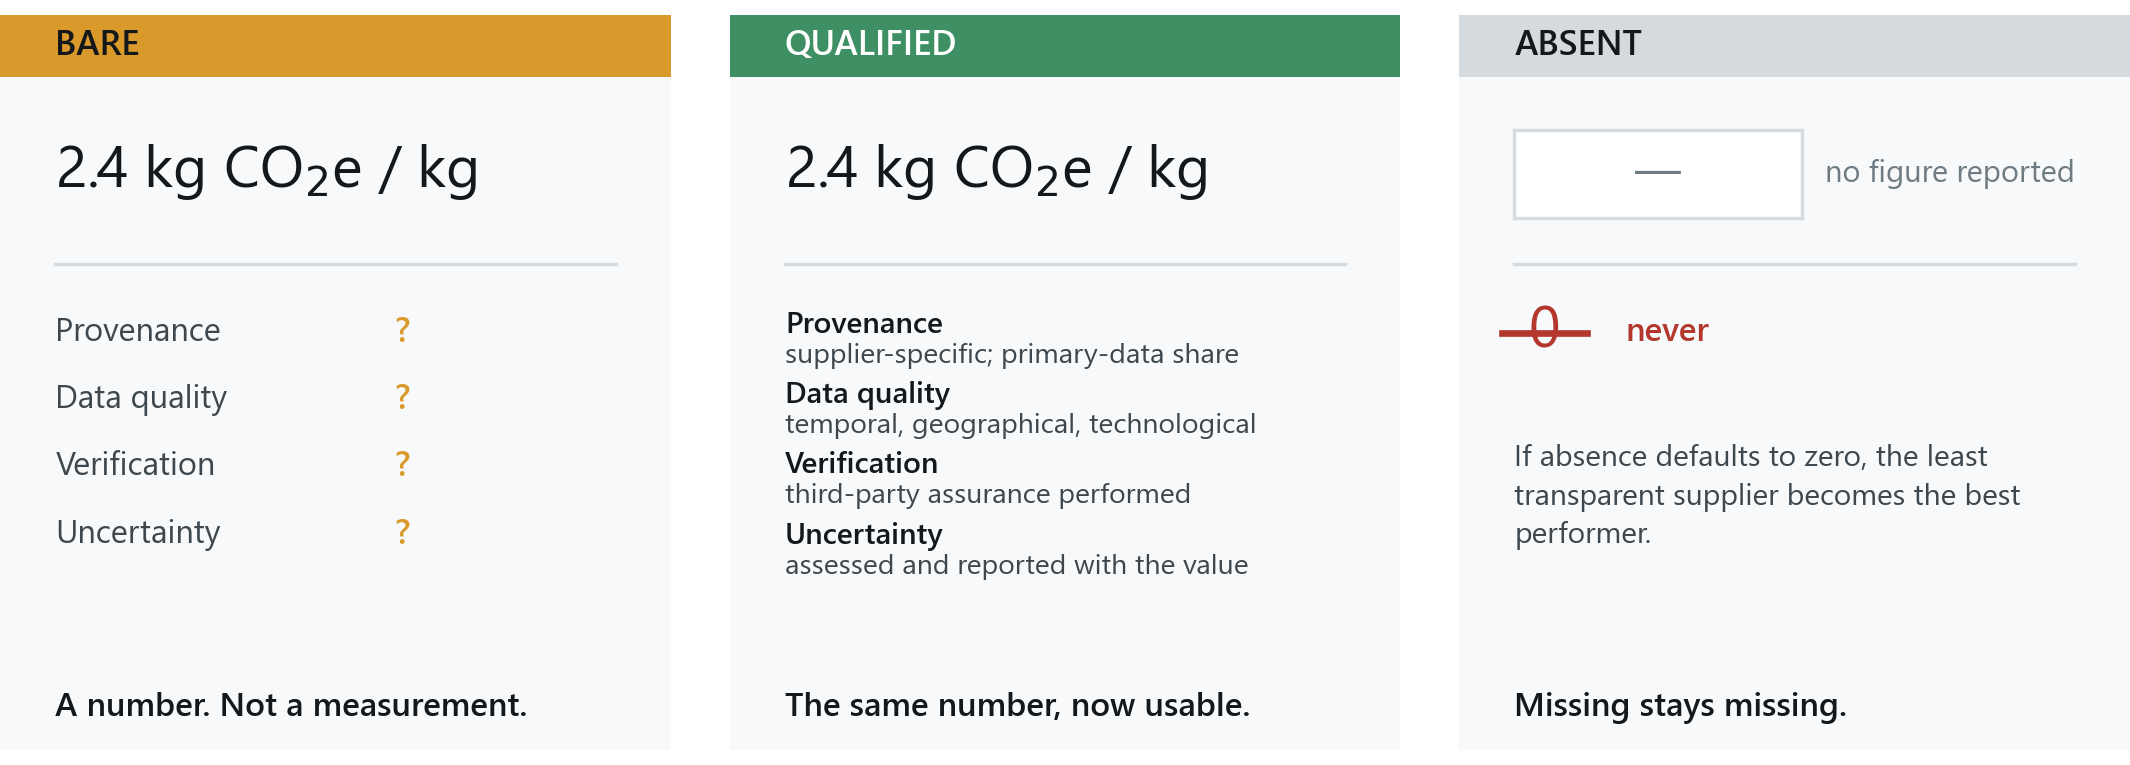
\includegraphics[width=\textwidth]{figures/fig03_evidence_chain.png}
  \caption{The same value in three states. \emph{Bare}: a figure without the
  relevant evidence attributes is not yet usable in a comparison. \emph{Qualified}: the same figure
  with provenance, data quality, verification and uncertainty attached becomes
  usable in a comparison. \emph{Absent}: no figure was reported, and the cell
  stays empty --- because if absence defaults to zero, the least transparent
  supplier becomes the best performer. The value shown is illustrative and is not
  taken from the dataset.}
  \label{fig:evidence}
\end{figure*}

Evidence quality is routinely treated as one attribute. The structure used
operationally throughout this paper separates four, each supported by the cited
sources (Figure~\ref{fig:evidence}): \emph{provenance} --- where the number came from;
\emph{data quality} --- how representative it is in time, geography and
technology \cite{a2}; \emph{verification} --- whether anyone independent checked
it; and \emph{uncertainty} --- how far apart two figures could actually be
\cite{p1}. None of the four may be blended into the performance number. A
quality-adjusted PCF destroys both the measurement and the evidence statement.

Two distinctions are easy to lose. \emph{Supplier-specific} and \emph{primary}
are not synonyms: a supplier-specific footprint normally combines primary
activity data with secondary background factors --- which is exactly why PACT
reports a \emph{share} of primary data rather than a flag \cite{p3,b2}. And an
industry-average emission factor, however recent, cannot by construction
distinguish two suppliers operating within the same industry.

\paragraph{Missing is never zero.} A missing environmental figure is a reportable
state, not a value. Substituting zero inverts the incentive structure of the
entire exercise: the supplier that discloses least obtains the best apparent
result. In the demonstrator this rule is enforced at four independent layers ---
in the measure definitions, in conditional formatting, in the figure-generation
code and in the absence of any imputation step in the pipeline --- so that no
single change can quietly reintroduce zero-filling.

\subsection{Materiality beyond carbon}
\label{sec:materiality}

Not every dimension matters for every material. A universal environmental data
request produces effort rather than decisions. The organising question is
materiality: \emph{could this dimension materially change the decision for this
material, from this feedstock, from this origin?}

The answer varies by driver, not by fashion. Water impacts are basin-specific, so
a generic per-kg water league table is methodologically wrong even where data
exists \cite{v3}. Land use and biodiversity pressure attach to feedstock and
origin rather than to the delivered kilogram. Circularity outcomes depend on
material, feedstock and application \cite{p2}. Climate is the exception that
proves the rule: it is in scope for every material in this project's scope, which
is why it is the dimension the prototype measures. Everything else enters the
decision only where the screening question above returns yes for the specific
material, feedstock and origin; the class column of
Table~\ref{tab:dimensions} records where each dimension sits for the material
groups in this project.

% ═══════════════════════════════════════════════════════════════════════
\section{Practices and how well each is evidenced}
\label{sec:practices}

Thirteen practices emerged from the underlying research, organised along the
decision sequence and shown in Table~\ref{tab:practices}. Four of them are
strongly evidenced, resting on a primary standard or an EU authority read in the
original. The remainder are supported by narrower citations, and one is an
explicit project recommendation.

Showing which is which is itself a practice. A benchmark method that presents a
plausible recommendation with the same authority as a standard requirement
invites the reader to over-trust both. The three-state marker used in
Table~\ref{tab:practices} describes only \emph{how well a practice is supported}.
It is not a maturity level, it does not describe an organisation, and no score is
computed from it.

\begin{table*}[t]
  \caption{Thirteen practices across the decision sequence, with the strength of
  the evidence behind each. $\blacksquare$~strongly evidenced --- primary standard
  or EU authority; $\square$~supported --- cited but narrower; $\triangle$~project
  recommendation --- plausible, not externally evidenced. The marker describes the
  support for the practice, never organisational maturity.}
  \label{tab:practices}
  \small
  \begin{tabular}{@{}p{0.075\textwidth}p{0.038\textwidth}p{0.030\textwidth}p{0.44\textwidth}p{0.33\textwidth}@{}}
    \toprule
    \dimhead{Step} & & & \dimhead{Practice} & \dimhead{Basis} \\
    \midrule
    \textsc{screen}  & $\square$    & & Screen on hard constraints first, and keep what was screened out visible & Constraints vs objectives \cite{c6} \\
                     & $\square$    & & Gate on specific legal or policy thresholds, not on general risk & \cite{v2,p5} \\
                     & $\square$    & & Treat supply risk as a dimension, not a footnote & \cite{a3,c5} \\
    \addlinespace[2pt]
    \textsc{compare} & $\blacksquare$ & & Define equivalent function before any per-kg benchmark & \cite{p1} \S A.1 \\
                     & $\blacksquare$ & & Satisfy the six comparability conditions before comparing suppliers & \cite{p1} \S A.1, Table A.2 \\
                     & $\square$    & & Require the primary-data share, not merely a supplier figure & \cite{p3,b2} \\
                     & $\square$    & & Declare a comparability verdict, not a confidence colour & \cite{p1,p3} \\
    \addlinespace[2pt]
    \textsc{qualify} & $\blacksquare$ & & Carry evidence quality beside the number, never inside it & \cite{a2,p3} \\
                     & $\blacksquare$ & & Never substitute zero for missing environmental data & \cite{a2,e2} \\
    \addlinespace[2pt]
    \textsc{decide}  & $\square$    & & Decide on total cost, not on price per kg & \cite{a1} \\
                     & $\square$    & & Price in regulatory cost transmission before it arrives & \cite{a7,a6} \\
                     & $\square$    & & Validate circularity against life-cycle impact & \cite{p2,c1} \\
    \addlinespace[2pt]
    \textsc{record}  & $\triangle$  & & One decision record for procurement and engineering, not two & \cite{a1} and construction \\
    \bottomrule
  \end{tabular}
\end{table*}

What a procurement organisation does differently, stated as compactly as the
evidence allows: name the rulebook in the request for quotation; require the
primary-data share; keep evidence beside the number; never zero-fill a gap; and
keep one decision record per case rather than two.

% ═══════════════════════════════════════════════════════════════════════
\section{Synthetic dataset and harmonisation}
\label{sec:data}

\begin{figure*}[t]
  \centering
  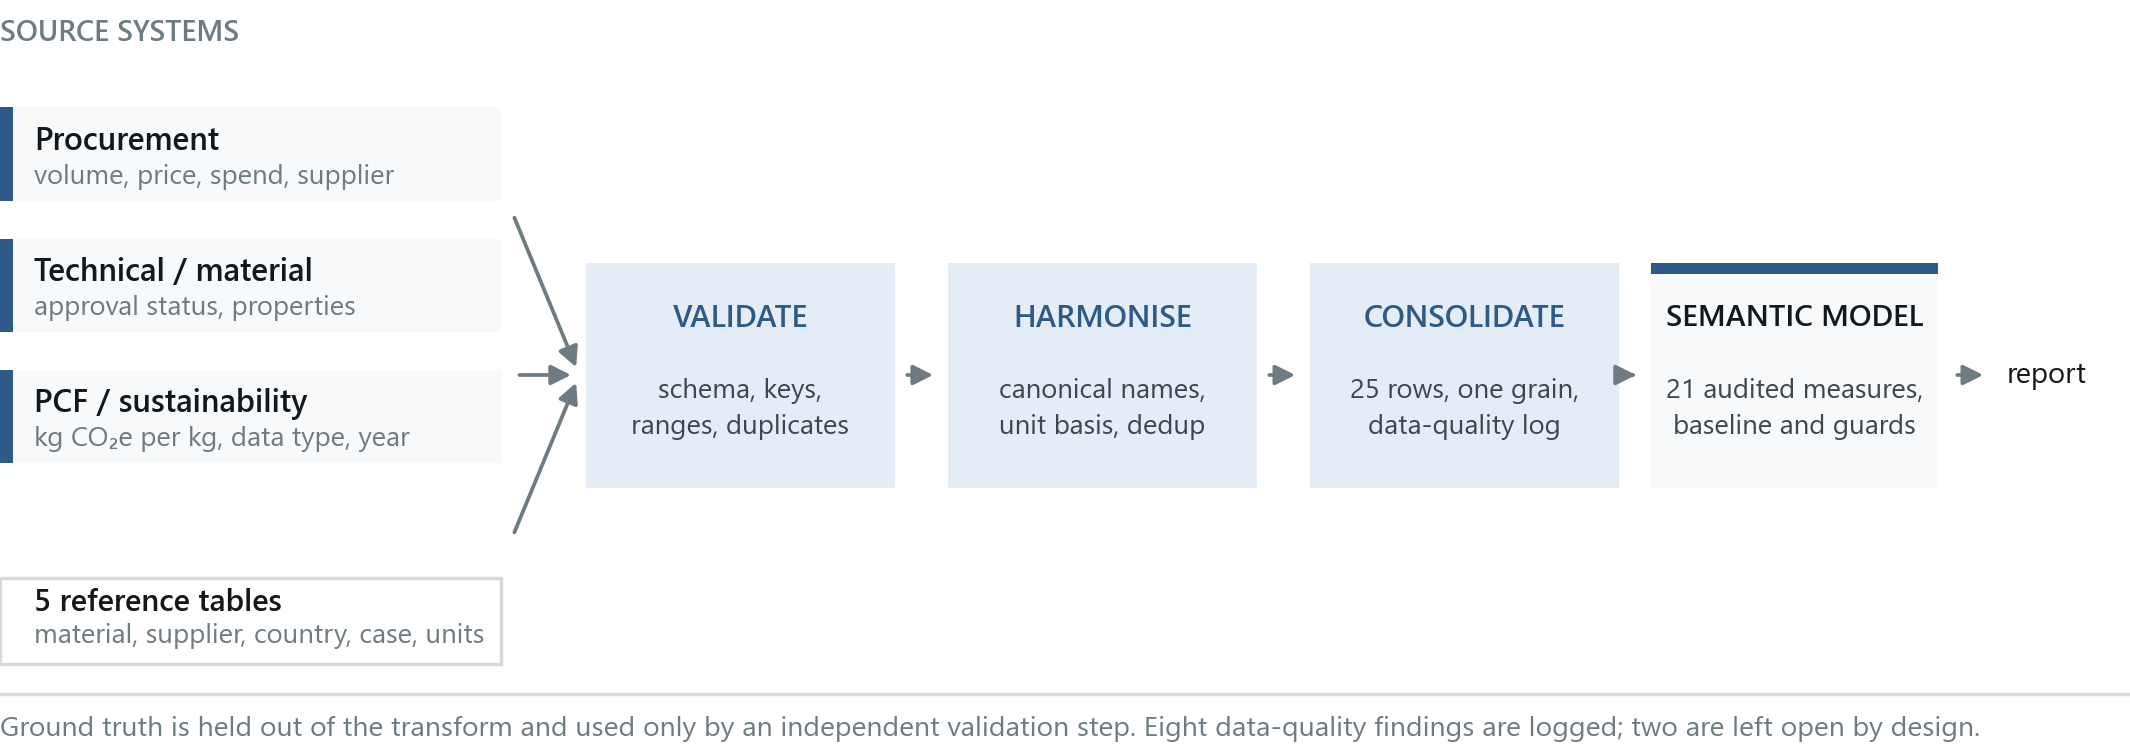
\includegraphics[width=\textwidth]{figures/fig04_data_lineage.png}
  \caption{Data lineage of the demonstrator. Three heterogeneous source extracts
  and five reference tables are validated, harmonised and consolidated into a
  single 25-row analytical grain, then exposed through an audited semantic layer.
  Ground truth is deliberately held out of the transform and read only by an
  independent validation step, so that the transform cannot be tuned to its own
  answer. \synth}
  \label{fig:lineage}
\end{figure*}

\subsection{Design}

The dataset describes five benchmark cases --- base oils, solvents, surfactants,
polymer additives, resins and binders --- each containing one incumbent and four
alternatives, giving 25 material rows. It is authored, not sampled. Every value
is synthetic, and no supplier, company or market data is used or implied
anywhere in the project.

Authoring the data is what makes the demonstration honest rather than
merely plausible. Because the defects were placed deliberately, the paper can
show the method meeting them, and a reader can verify from the repository that
nothing was cleaned away quietly.

\subsection{The data-quality problems, and which were left open}

Three source extracts arrive in the shape real ones do: a procurement extract, a
technical/material extract and a PCF extract, each with its own naming and its
own idea of a supplier identifier. Eight findings were logged
(Table~\ref{tab:dq}). Six were resolved deterministically through reference
tables --- never by fuzzy matching, so the resolution is reproducible and
auditable. Two were left open \emph{by design}, because they are the conditions
the analytical layer must be able to survive: one material has no PCF at all, and
one carries a PCF from an outdated reference year.

\begin{table*}[t]
  \caption{The data-quality log. Six findings are resolved deterministically
  through reference tables; two are left open by design because they are the
  states the method must handle rather than remove. Leaving them open is what
  makes the missing-value and evidence-quality behaviour observable downstream.
  \synth}
  \label{tab:dq}
  \small
  \begin{tabular}{@{}p{0.235\textwidth}p{0.115\textwidth}p{0.075\textwidth}p{0.50\textwidth}@{}}
    \toprule
    \dimhead{Finding} & \dimhead{Source} & \dimhead{Status} & \dimhead{Resolution} \\
    \midrule
    Duplicate procurement record & Procurement & resolved & Vendor-code migration produced a second row for one material--supplier relationship; deduplicated against the technical source's identifier \\
    Material naming inconsistency & Procurement & resolved & Free-text description mapped to the canonical name by exact lookup \\
    Material naming inconsistency & PCF & resolved & As above \\
    Supplier naming inconsistency & PCF & resolved & Legal-form and spelling variants mapped to the canonical supplier \\
    Country representation inconsistency & PCF & resolved & Country name and code variants mapped to a single representation \\
    PCF unit basis inconsistency & PCF & resolved & Values reported per tonne converted to the per-kilogram basis before consolidation \\
    \addlinespace[2pt]
    \textcolor{pamber}{\textbf{Missing PCF value}} & PCF & \textcolor{pamber}{\textbf{open}} & One material has no reported PCF. Left missing: it is excluded from the carbon comparison and retained in every other \\
    \textcolor{pamber}{\textbf{Outdated PCF reference year}} & PCF & \textcolor{pamber}{\textbf{open}} & One material carries a 2019 industry-average factor. Left in place and flagged, because suppressing it would hide the evidence problem \\
    \bottomrule
  \end{tabular}
\end{table*}

\subsection{Pipeline and independent validation}

The pipeline (Figure~\ref{fig:lineage}) is deterministic: given the same inputs it
produces the same consolidated dataset and the same log. Its most important
property is structural. A ground-truth version of the consolidated dataset exists
in the repository, and the transform never reads it; validation is a separate step
that compares the transform's output against ground truth after the fact. A
transform with access to the expected answer can be tuned until it agrees, which
demonstrates nothing.

\subsection{Semantic layer}

The consolidated dataset is exposed through 21 audited measures. Three design
decisions in that layer carry the method:

\begin{itemize}
  \item \textbf{Baseline by case.} The incumbent baseline is resolved within the
        current case, so a delta is always against the right reference and never
        against a portfolio average.
  \item \textbf{A grain guard.} Percentage measures return blank unless a single
        material is in context. This makes a cross-case aggregate percentage
        structurally impossible rather than merely discouraged.
  \item \textbf{No imputation.} There is no coalesce-to-zero anywhere in the
        layer, so a missing PCF propagates as missing into every dependent
        measure and every visual.
\end{itemize}

One defect found during the audit is worth reporting because it is
characteristic. Numeric columns had been typed without an explicit locale, and
under a German-locale engine a value such as \texttt{240000.0} was parsed as
240{,}000{,}000 --- a silent factor-of-ten class of error across several columns.
It was corrected by making the locale explicit at every conversion step. The
lesson generalises: in a benchmarking pipeline, a plausible wrong number is more
dangerous than a missing one.

% ═══════════════════════════════════════════════════════════════════════
\section{The analytics prototype}
\label{sec:prototype}

The semantic layer is displayed through a three-page interactive report: a
portfolio overview, a material-level decision analysis and a portfolio screening
matrix. Three behaviours distinguish it from a conventional supplier dashboard.

Gates are \emph{shown, never applied as a filter}. A blocked alternative remains
on every page with its block reason attached. A dashboard that filters out
ineligible options hides the most valuable finding in the dataset, as
Section~\ref{sec:results} shows.

Evidence sits beside performance in its own columns --- provenance, reference
year and a data-quality tier --- and is never folded into the performance figure.
The tier is a prototype design heuristic derived from provenance and recency, and
is labelled as such; it is not a standards-conformant data-quality assessment.

Missing values are rendered as missing. Where a carbon delta is undefined the cell
reads \emph{n/a}, in the same visual weight as any other cell, rather than as a
zero or a gap in a bar.

% ═══════════════════════════════════════════════════════════════════════
\section{Results}
\label{sec:results}

The deltas below demonstrate the method's behaviour, not a validated supplier
comparison. Measured against the six conditions of
Section~\ref{sec:comparability}, the comparisons are at best conditional, as
Section~\ref{sec:boundary} sets out.

\subsection{The portfolio total is not the sum of the options}

The first result is arithmetic rather than environmental. Summing the annual spend
of all 25 rows gives \eur{4{,}073{,}400}. That figure is meaningless as a
portfolio position, because the four alternatives in each case are mutually
exclusive scenarios for the same demand: summing them counts that demand five
times over. The position actually held is the incumbent portfolio ---
\eur{820{,}000} of annual spend, 480{,}000~kg of annual volume and 605{,}000~kg
of annual \co{}. The naive total overstates the portfolio by a factor of
approximately five.

This is the kind of error that a scorecard with more columns does not prevent and
a correctly specified baseline measure does. Coverage across the 25 rows is
likewise reported rather than assumed: 23 of 25 alternatives are technically
eligible (92.0\%), 24 of 25 carry a PCF (96.0\%), and 96.8\% of spend is covered
by a PCF.

\subsection{All alternatives on one surface}

\begin{sidewaysfigure*}
  \centering
  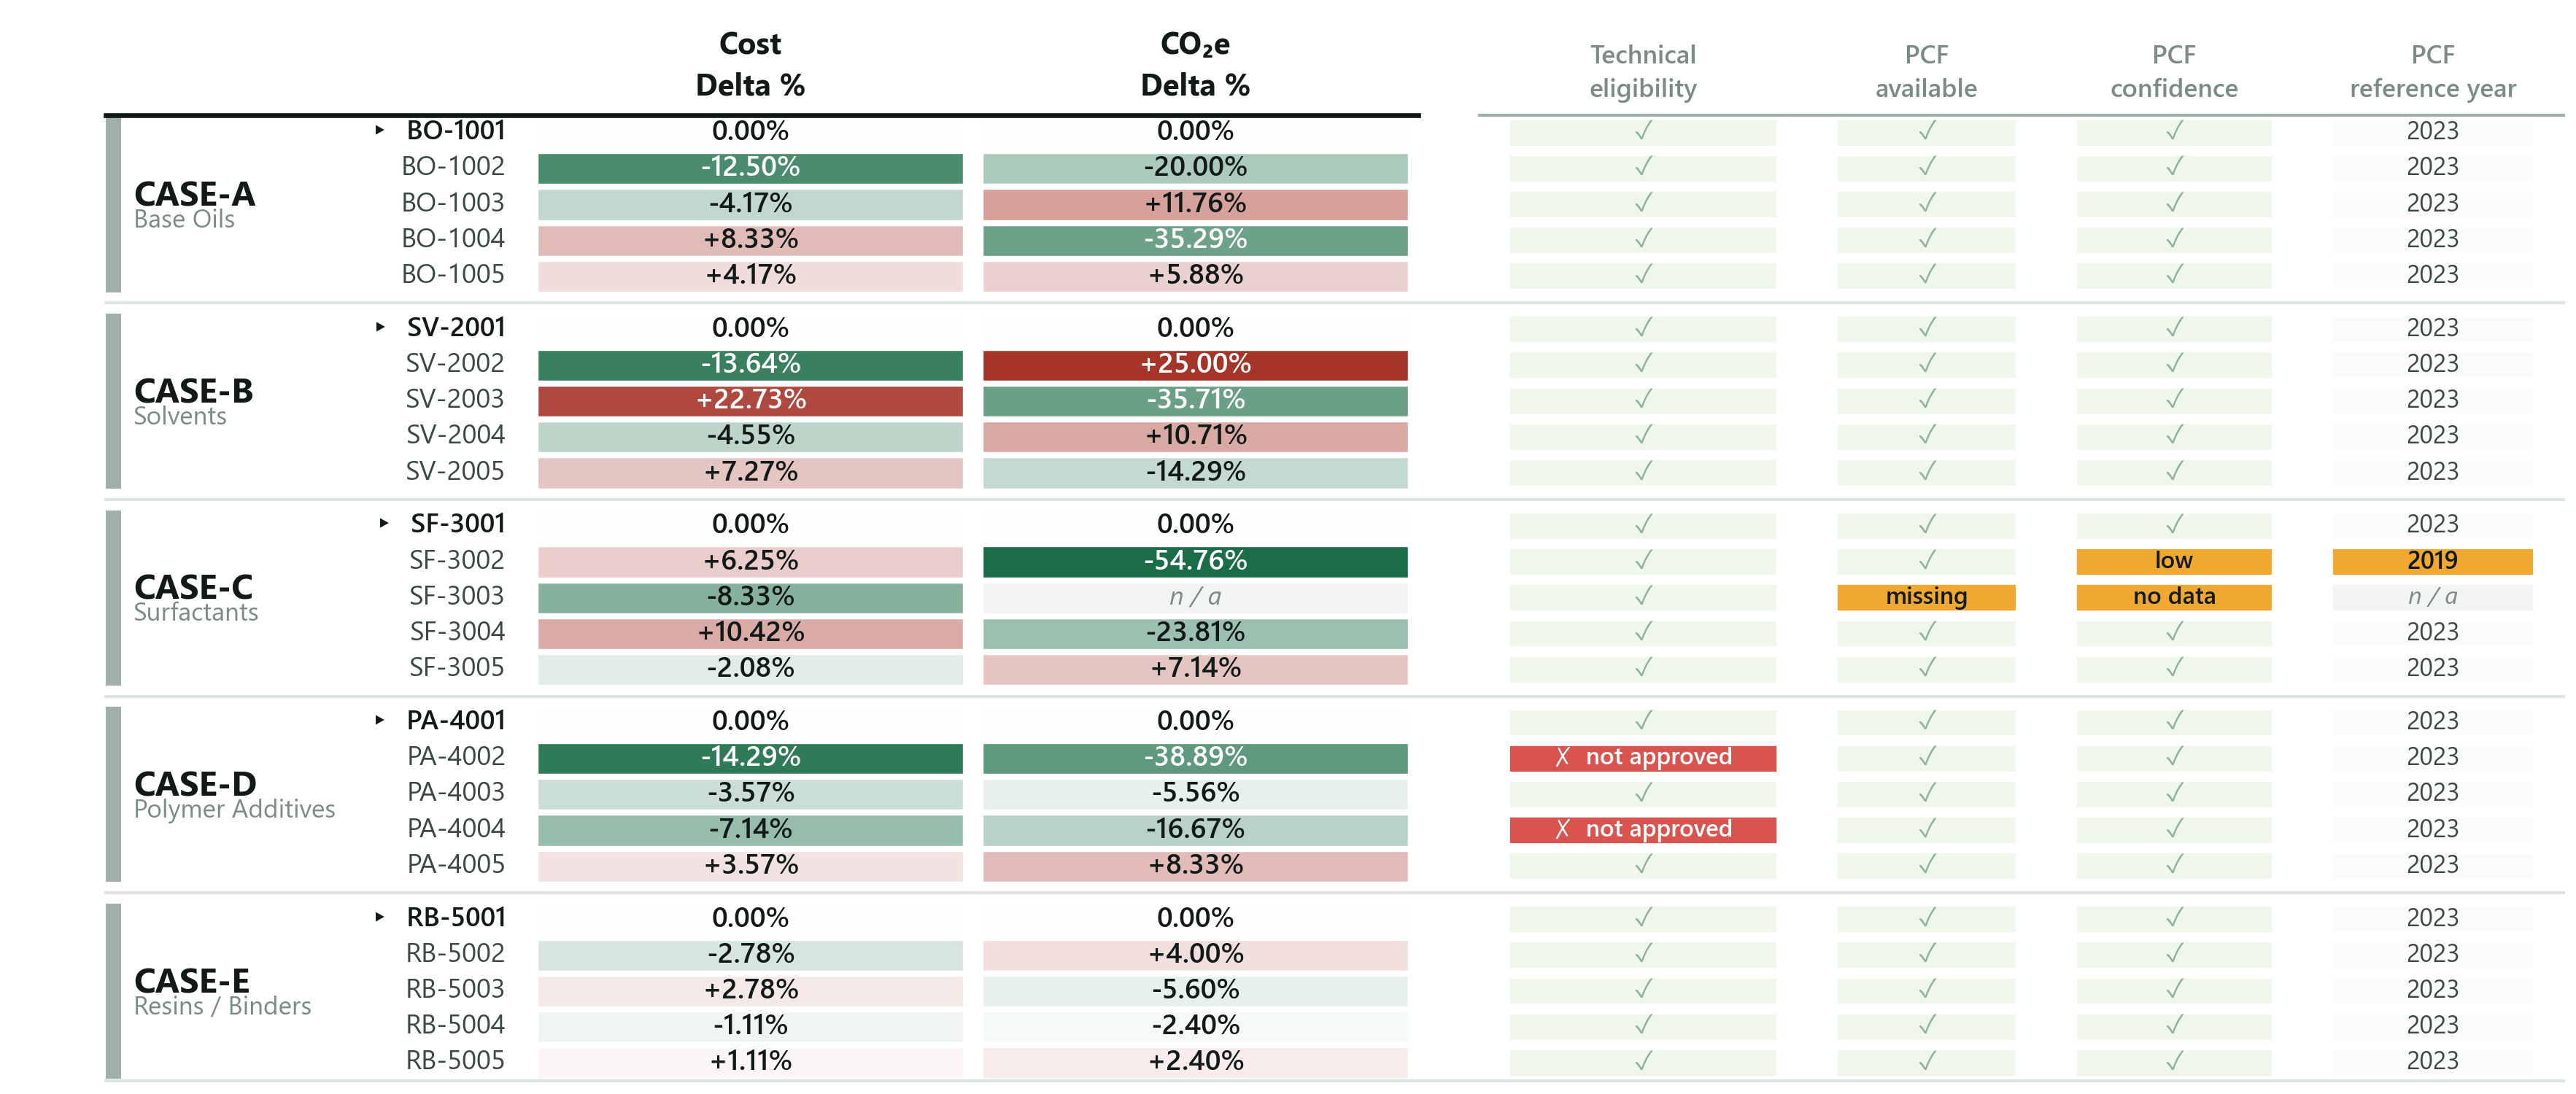
\includegraphics[width=0.97\textheight]{figures/fig05_portfolio_heatmap.png}
  \caption{Portfolio screening across all 25 alternatives and five benchmark
  cases. Cost and \co{} deltas are the analysis; technical eligibility and the
  three evidence columns are exceptions, shown recessed until they are not normal.
  Colour compares each material with the incumbent \emph{of its own case}, and each
  case is an independent decision --- the surface is a screen, not a league table.
  \emph{n/a} means the value is unknown and is never read as zero;
  $\blacktriangleright$ marks the incumbent. No score, no ranking and no weighting
  is derived. \synth}
  \label{fig:heatmap}
\end{sidewaysfigure*}

Figure~\ref{fig:heatmap} places every alternative on one surface. The design
carries three of the method's commitments simultaneously. The two performance
columns are visually dominant and diverge around the incumbent at zero. The four
status columns recede to a pale tint when normal and become explicit only as
exceptions --- red for a technical blocker, amber for weak, outdated or missing
evidence. And the missing carbon figure for SF-3003 is present as \emph{n/a},
occupying its cell rather than vanishing from it.

Read as a screen, the surface answers one question per case rather than one
question overall. That constraint is not a limitation of the visualisation; it is
the analytical claim. It applies the same benchmarking principle as
Figure~\ref{fig:profile} at portfolio scale: the dimensions stay separate, each
is compared against its own reference, and no total is formed.

\subsection{CASE-D: performance cannot buy eligibility}

\begin{figure}[htb]
  \centering
  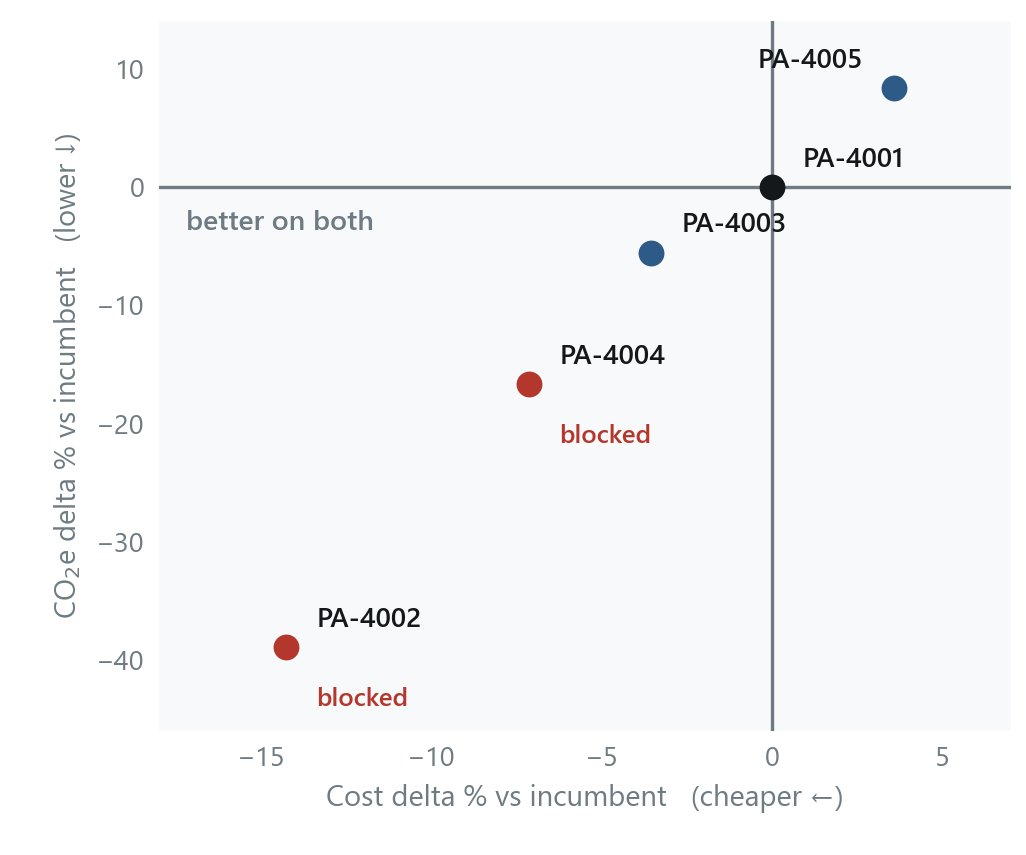
\includegraphics[width=\columnwidth]{figures/fig06_case_d_quadrant.png}
  \caption{CASE-D on cost and carbon. The two alternatives furthest into the
  better-on-both quadrant, PA-4002 and PA-4004, are both technically blocked. The
  only eligible improvement is PA-4003, at a fraction of the apparent
  opportunity. \synth}
  \label{fig:cased}
\end{figure}

In the polymer additives case, the ranking on cost and carbon looks unambiguous.
PA-4002 is 14.29\% cheaper and 38.89\% lower in \co{} than the incumbent; PA-4004
is 7.14\% cheaper and 16.67\% lower. Both are technically blocked --- PA-4002 is
not approved, PA-4004 is under qualification --- and neither can be bought today.

The only eligible improvement is PA-4003, at $-3.57\%$ on cost and $-5.56\%$ on
\co{}: real, but a small fraction of the apparent opportunity. That, and not
$-14.29\%$, is the decision actually on the table.

Two consequences follow. First, performance cannot compensate for failed
eligibility; a gate is passed or it is not. Second, the blocked options must stay
visible with their reasons, because PA-4004 is under qualification and may return
--- which converts a screening result into a qualification-pipeline question with
a date and an owner.

\subsection{CASE-C: the best result on the weakest evidence}

In the surfactants case all five materials are technically approved, so
eligibility settles nothing and evidence settles everything
(Table~\ref{tab:casec}).

SF-3002 shows the strongest carbon result in this case at $-54.76\%$.
It rests on an industry-average factor from 2019, classified low confidence. The
figure is not wrong; it is simply not yet a supplier comparison, because an
industry-average factor cannot distinguish two suppliers inside the same industry.

SF-3003 is 8.33\% cheaper and has no carbon figure at all. It remains blank on
carbon in the measure, in the heatmap and in the case total. It is not zero, it is
not a poor performer, and it is not dropped from the cost comparison. It is
unknown, and it stays unknown.

\begin{table*}[t]
  \caption{CASE-C, all five materials. Performance and the confidence in that
  performance occupy separate columns, and the row with the strongest carbon
  result carries the weakest evidence. SF-3003 has no PCF: its carbon cells are
  empty rather than zero, and it remains in the cost comparison. \synth}
  \label{tab:casec}
  \small
  \begin{tabular}{@{}lrrrlrl@{}}
    \toprule
    \dimhead{Material} & \dimhead{Cost $\Delta$} & \dimhead{\co{} $\Delta$} &
    \dimhead{PCF} & \dimhead{PCF data type} & \dimhead{Year} & \dimhead{Confidence} \\
    \midrule
    SF-3001 & $0.00\%$ & $0.00\%$ & 2.10 & Supplier-specific (primary) & 2023 & High \\
    \textcolor{pamber}{\textbf{SF-3002}} & \textcolor{pamber}{$+6.25\%$} & \textcolor{pamber}{$\mathbf{-54.76\%}$} & \textcolor{pamber}{0.95} & \textcolor{pamber}{\textbf{Industry-average (secondary)}} & \textcolor{pamber}{\textbf{2019}} & \textcolor{pamber}{\textbf{Low}} \\
    \textbf{SF-3003} & $-8.33\%$ & --- & --- & \textbf{no PCF reported} & --- & \textbf{No data} \\
    SF-3004 & $+10.42\%$ & $-23.81\%$ & 1.60 & Supplier-specific (primary) & 2023 & High \\
    SF-3005 & $-2.08\%$ & $+7.14\%$ & 2.25 & Supplier-specific (primary) & 2023 & High \\
    \bottomrule
  \end{tabular}
\end{table*}

% ═══════════════════════════════════════════════════════════════════════
\section{Trade-offs and handling rules}
\label{sec:tradeoffs}

\subsection{Different tensions, different rules}

The tensions in a sourcing decision are structurally different from one another
(Table~\ref{tab:tradeoffs}). Some resolve at a gate. Some are genuine two-axis
trade-offs. One is about evidence rather than performance at all. Each has a
handling rule, and not one of the rules is a weight.

This matters because weighting is a common reflex. A weight asserts an
exchange rate between dimensions that the evidence does not supply, then hides
that assertion inside a total. Where an exchange rate is genuinely needed --- for
instance a cost per tonne of \co{} avoided --- it should be displayed as a ratio
so that it can be argued with, not embedded in a score.

\begin{table*}[t]
  \caption{The trade-off map. Eight tensions, each with the way it appears in a
  decision and the rule that handles it. Evidence strength uses the same
  three-state marker as Table~\ref{tab:practices}. Cost--carbon quantitative
  evidence is steel-sector illustration only; no chemical-sector figure was
  retrieved, which is why that row carries the weakest marker.}
  \label{tab:tradeoffs}
  \small
  \begin{tabular}{@{}p{0.225\textwidth}p{0.030\textwidth}p{0.295\textwidth}p{0.375\textwidth}@{}}
    \toprule
    \dimhead{Tension} & & \dimhead{How it appears} & \dimhead{Handling rule} \\
    \midrule
    Cost $\leftrightarrow$ carbon & $\triangle$ & The cheaper option carries more carbon, or the reverse & Two axes, plus a displayed cost-per-tonne ratio --- never a score \\
    Circularity $\leftrightarrow$ non-climate impacts & $\blacksquare$ & Recovery wins on climate and loses elsewhere & Report as distinct outputs; any priority rule is stated per case \\
    Circularity $\leftrightarrow$ technical performance & $\square$ & Recycled content shifts the specification & Gate --- recycled content is a candidate only if it passes equivalence \\
    Circularity $\leftrightarrow$ cost & $\square$ & The break-even arrives later than the target date & Treat the horizon as an explicit scenario, not an assumption \\
    Sustainability $\leftrightarrow$ technical performance & $\blacksquare$ & A carbon gain sits behind a failed approval & Gate. No carbon result buys past a technical blocker \\
    Sustainability $\leftrightarrow$ supply security & $\square$ & A carbon gain raises supplier concentration & State it beside the result; concentration needs awarded volumes \\
    Performance $\leftrightarrow$ evidence quality & $\blacksquare$ & The best number has the weakest provenance & Two columns. Never a quality-adjusted performance figure \\
    Carbon $\leftrightarrow$ other environmental burdens & $\blacksquare$ & A GHG-only view misses the shift & Disclose scope. Methods exist \cite{v3,v4}; the constraint is supplier data \\
    \bottomrule
  \end{tabular}
\end{table*}

\subsection{Circularity is not automatically an improvement}

\textbf{Scope, stated before the finding: the following is a plastics
waste-treatment study. It demonstrates a mechanism --- burden shifting between
impact categories --- and is not evidence about base oils, solvents, surfactants,
polymer additives or resins.}

A European Commission JRC assessment \cite{p2} compared 27 recycling pathways
across 14 impact categories. Recycling beat energy recovery on climate in every
pathway analysed. On five other categories --- acidification, particulate matter,
ionising radiation, human toxicity (non-cancer) and eutrophication --- energy
recovery can perform better than energy-intensive recycling routes, and the
assessment names those routes: PET alkaline hydrolysis, PS mechanical, MPO
mechanical and pyrolysis, PE film mechanical and physical, and EPS physical
recycling.

Three further findings from the same source matter for a benchmark method:
technical quality issues in the recovered material; negative net incomes for
methanolysis, pyrolysis and gasification; and, across the whole study, that ``a
clear ranking could not be established''. The result is also conditional on the
European electricity mix, and the assessment states that as the mix decarbonises
the gap widens further in favour of recycling. A circularity conclusion therefore
carries a date.

The methodological consequence is direct. A universal ordering --- impact first,
circularity second, or the reverse --- is not supported. Circularity and
life-cycle impact are assessed as distinct outputs, hard constraints are applied
first, and any priority rule is made explicit for the specific case rather than
applied as policy.

% ═══════════════════════════════════════════════════════════════════════
\section{Governance and decision ownership}
\label{sec:governance}

Every practice in this paper fails at the same seam. Engineering owns the gates,
procurement owns the commercial comparison, sustainability owns the evidence
rules, compliance owns the legal thresholds --- and each function keeps its own
list. ISO~20400 addresses exactly this by placing sustainability criteria
alongside price and quality inside one evaluation rather than in a parallel
process \cite{a1}.

\textbf{The following ownership split and record design are a project synthesis
and a design recommendation.} ISO~20400 supports the principle; it does not
validate this artefact.

Engineering defines the function and validates technical equivalence. Procurement
owns commercial terms, capacity evidence and sourcing scenarios. Sustainability
defines accepted methods and evidence requirements. Compliance defines the
specific legal and policy gates and runs the due-diligence risk process.
Suppliers provide declarations and evidence but never self-approve gate status. A
named business decision owner accepts the residual trade-off, on the record.

The artefact that makes this operable is one decision record per benchmark case,
carrying: incumbent and candidates; gate status with the reason, blocked options
still visible; cost position and carbon position on separate axes; evidence status
per number; the comparability verdict; the decision and what was given up; the
named owner; and a review date. A second output falls out of the same record and
should not be buried in it --- the qualification pipeline: which blocked
candidates are worth qualifying, by when, and at whose cost.

The prototype is not yet this artefact. Its material-level page is the closest
existing approximation: it displays the decision context but captures neither the
decision, nor the owner, nor the review date.

% ═══════════════════════════════════════════════════════════════════════
\section{Scope boundary}
\label{sec:boundary}

The honest headline for the demonstrator is that its architecture is the right
shape while the comparison it performs is not yet demonstrably valid ---
and that the conditions for making it valid are known and enumerable.

Measured against the six conditions of Section~\ref{sec:comparability}: the unit
of analysis is a declared per-kilogram unit with no functional normalisation,
although the dataset's own active-content variation shows the materials are not
functionally identical per kilogram; there is no boundary or data-period field; no
methodology rulebook or version is recorded; provenance and a data-quality tier
are present, but the primary-data share and any uncertainty statement are absent;
representativeness is temporal only, through a reference year; and there is no
verification field at all. \textbf{No condition is fully satisfied today.}

Eight fields would close the gap, and all eight are collected upstream in the
specification and the request for quotation rather than repaired downstream in
the analysis: a functional or declared unit with its reference flow; the
methodology rulebook and version; a boundary description or comparability flag;
the primary-data share; verification status and scope; the data or reference
period; an uncertainty statement; and the comparability verdict itself.

Naming these is not an admission that weakens the demonstrator. It is what
converts it from a picture into a specification.

% ═══════════════════════════════════════════════════════════════════════
\section{Discussion}

The recurring objection to a method without a score is that executives want one
number. The evidence assembled here suggests that the single number is not
available at the price usually assumed. A composite requires an exchange rate
between dimensions; an EU authority running a full life-cycle and life-cycle-cost
assessment across 27 pathways and 14 categories concluded that ``a clear ranking
could not be established'' \cite{p2}. If that ranking could not be established
with a complete inventory, it will not be established by weighting four columns
of partially populated supplier data.

What a sequence buys instead is decision-grade failure. Each step produces a
statement that can be argued with: this option is not eligible, and here is the
threshold and its owner; these two figures are conditionally comparable, and here
is the condition that is unmet; this improvement is real but rests on a 2019
industry-average factor. A composite converts all three into the same thing --- a
slightly lower score --- and destroys the information that would have driven an
action.

The demonstrator also shows that the expensive properties are structural rather
than cosmetic. Gates that screen without deleting, evidence carried beside
performance, missing values preserved, and cases kept independent are all choices
that are cheap to make at design time and very hard to retrofit once an
aggregate exists. Adding a comparability verdict to this architecture is a
data-collection task. Removing an embedded weighting from a deployed scorecard is
an organisational one.

% ═══════════════════════════════════════════════════════════════════════
\section{Limitations}
\label{sec:limits}

\paragraph{Evidence limitations.} No industrial chemical-procurement case
supports the framework; the demonstration is synthetic throughout. No empirical
study was found quantifying how far real supplier PCFs diverge when the \S A.1
conditions are violated, so the size of the comparability problem is argued
structurally rather than measured. TfS~v3 and Catena-X~v4 were not read in full,
and are cited as examples of the additional programme specifications the standard
requires, not as verified conformance targets. No chemical-sector green-premium
dataset was retrieved; the cost--carbon exchange-rate evidence is steel-sector
illustration only. No company-level supply-resilience metric set was retrieved.
The GHG~Protocol \emph{Product Standard} dates from 2011 while a joint ISO/GHG
Protocol product-standard process was reported active in 2026.

Access depth is disclosed per source in the reference list. Five primary sources
were read in the original at section level; the majority of the remaining entries
were read at summary level, and the paper's claims are calibrated accordingly.

\paragraph{Method limitations.} The four-role convention and the trade-off map are
project syntheses. The three-state comparability verdict is a source-supported
interpretation of the standard's conditions, not a provision of the standard.
The dimensions in Table~\ref{tab:dimensions} are a working set for this
project's material groups, not a fixed or universal list. Roles are not mutually
exclusive: supply risk can be a gate, a performance dimension or context
depending on the decision rule in force.

\paragraph{Demonstrator limitations.} The prototype's data-quality tier is a
design heuristic derived from provenance and recency, not a standards-conformant
data-quality assessment. Coverage percentages are computed against the project's
own inventory and weight unequal items equally. Supplier concentration is not
derivable from the dataset, because mutually exclusive scenarios carry no awarded
volumes. And, as Section~\ref{sec:boundary} states, no \S A.1 condition is fully
satisfied.

% ═══════════════════════════════════════════════════════════════════════
\section{Future work}

Two build lanes follow, and one list is a refusal.

\textbf{Lane A --- make the existing comparison defensible.} Add the eight fields
of Section~\ref{sec:boundary}. This stays inside the analytical question the
prototype already asks and is the only work that changes the validity of its
current output.

\textbf{Lane B --- add category modules where materiality justifies them.}
Recycled and renewable content with a chain-of-custody model \cite{v5};
due-diligence and human-rights performance; hazardous-substance legal status;
criticality and supply resilience; water, land use, biodiversity, pollution and
toxicity; and CBAM exposure where a product code falls outside current scope.
Each is gated by the materiality question of Section~\ref{sec:materiality} and
each needs its own data owner and grain.

\textbf{Do not build until real data exists.} Qualification and switching cost;
true total-cost effects on yield, energy, quality and downtime; supplier capacity,
ramp-up and recovery time; country or supplier concentration on awarded shares;
toxicity and legal use status for actual substances and applications; recycled or
renewable chain-of-custody and mass-balance claims; and responsible-sourcing
findings. Synthesising any of these would demonstrate columns rather than
capability, and would corrupt exactly the credibility the rest of the method is
built to protect.

% ═══════════════════════════════════════════════════════════════════════
\section{Conclusion}

This paper set out a method for comparing sustainable raw-material alternatives
that does not produce a sustainability score. The method is a sequence:
eligibility, then comparability, then evidence, then trade-off, then a recorded
decision with a named owner. Ten success dimensions give the decision context a
structured view, each read against a benchmark rather than combined. Four
decision roles keep gates, performance,
evidence and context from contaminating one another. Six standard conditions
decide whether two supplier carbon figures may be compared at all, and a
three-state verdict reports the answer.

Demonstrated on 25 synthetic alternatives across five independent cases, the
method surfaced findings that a scorecard would have hidden: a portfolio total
overstated approximately fivefold, two leading candidates that cannot be bought, a
best-in-portfolio carbon result resting on a 2019 industry-average factor, and one
material that has no carbon figure and is never given one.

The demonstrator does not prove comparability, and the paper says so and names the
eight fields that would. That boundary is the contribution as much as the method
is. A benchmark that reports what it cannot yet support is more useful to a
sourcing decision than one that reports a number it cannot defend.

% ═══════════════════════════════════════════════════════════════════════
\begin{thebibliography}{99}\small
\setlength{\itemsep}{1.5pt}

\bibitem{p1} WRI \& WBCSD (GHG Protocol). \emph{Product Life Cycle Accounting and
Reporting Standard}. 2011. \ev{[full text: \S1.2, \S1.5--\S1.7, Appendix A \S A.1, Table A.2]}

\bibitem{p2} Garcia-Gutierrez, P.; Amadei, A.\,M.; Klenert, D.; Nessi, S.;
Tonini, D.; Tosches, D.; Ardente, F.; Saveyn, H. \emph{Environmental and economic
assessment of plastic waste recycling}. European Commission, Joint Research
Centre, JRC132067, 2023. \ev{[full text: executive summary]}

\bibitem{p3} WBCSD / PACT. \emph{PACT Methodology v3.0}. 2025. \ev{[full text]}

\bibitem{p4} European Chemicals Agency. \emph{Guidance on requirements for
substances in articles}, v3.0. 2015. \ev{[full text: title page, legal note, \S2--2.4]}

\bibitem{p5} European Parliament \& Council. Directive (EU) 2026/470 of 24
February 2026 amending Directives 2006/43/EC, 2013/34/EU, (EU) 2022/2464 and (EU)
2024/1760. 2026. \ev{[locator and operative dates confirmed]}

\bibitem{a1} ISO. \emph{ISO 20400 --- Sustainable procurement: Guidance}. 2017. \ev{[summary]}

\bibitem{a2} ISO / JRC / US EPA. ISO 14040 and 14044 data-quality requirements;
pedigree-matrix guidance. 2006, 2016--2017. \ev{[summary]}

\bibitem{a3} European Union. Regulation (EU) 2024/1252 --- Critical Raw Materials
Act. 2024. \ev{[summary]}

\bibitem{a4} European Commission / EFRAG. ESRS Set 1 --- Delegated Regulation
(EU) 2023/2772, topical standards E1--E5. 2023. \ev{[summary]}

\bibitem{a6} European Commission. Ecodesign for Sustainable Products Regulation
and Digital Product Passport. 2024--. \ev{[summary]}

\bibitem{a7} European Commission. Carbon Border Adjustment Mechanism ---
definitive period. 2026. \ev{[summary]}

\bibitem{b1} Together for Sustainability. \emph{Product Carbon Footprint
Guideline for the Chemical Industry}, v3.0; Data Model v3.1. 2024--2025. \ev{[summary]}

\bibitem{b2} WBCSD / PACT. \emph{PACT Methodology v3.0 and Technical
Specifications v3.0.3}. 2025. \ev{[full text]}

\bibitem{b3} Catena-X. \emph{Product Carbon Footprint Rulebook v4}. 2025. \ev{[summary]}

\bibitem{b6} OECD. \emph{Due Diligence Guidance for Responsible Business
Conduct}. 2018; 2023 update. \ev{[summary]}

\bibitem{c1} Halstenberg, F.\,A.; Lindow, K.; Stark, R. Leveraging Circular
Economy through a Methodology for Smart Service Systems Engineering. 2019.
\ev{[full text: introduction and background]}

\bibitem{c5} Materials selection in a critical raw materials perspective. 2019. \ev{[summary]}

\bibitem{c6} Optimizing lightweight material selection in automotive
engineering: a hybrid Ashby--VIKOR approach. 2025. \ev{[summary]}

\bibitem{c7} Data quality and uncertainty assessment of life-cycle inventory data
for composites. 2024. \ev{[summary]}

\bibitem{d1} BASF. \emph{Methodology for Product Carbon Footprint Calculation}.
Current. \ev{[summary]}

\bibitem{e2} Sphera. \emph{Supplier PCF Data: Overcoming Barriers and Driving
Decarbonization}. 2024--2025. \ev{[summary]}

\bibitem{v1} European Commission. Corporate sustainability due diligence ---
status after Directive (EU) 2026/470: in force 18 March 2026, transposition by
26 July 2028. \ev{[locator and operative dates confirmed]}

\bibitem{v2} European Chemicals Agency. \emph{Summary of obligations resulting
from inclusion of substances of very high concern in the Candidate List}.
\ev{[summary; Art. 3(3) definition verbatim from \cite{p4}]}

\bibitem{v3} ISO. \emph{ISO 14046:2014 --- Environmental management: Water
footprint. Principles, requirements and guidelines}. 2014. \ev{[catalogue record]}

\bibitem{v4} European Commission. Commission Recommendation (EU) 2021/2279 on the
use of the Environmental Footprint methods; 16 impact categories. 2021. \ev{[summary]}

\bibitem{v5} ISCC PLUS. Chain-of-custody and mass-balance bookkeeping.
\ev{[summary]}

\end{thebibliography}

\vspace{0.8em}
\noindent{\footnotesize\textcolor{ink3}{\textbf{Data and reproducibility.} All
data in this paper is synthetic. The dataset, the deterministic transformation and
validation scripts, the semantic-layer measure definitions and the generators for
every figure in this paper will be published with the project repository. Every
source used is listed above with the access depth at which it was read. No
supplier, company or market data is used or implied anywhere in the project.
\quad\textcopyright~2026 Csaba Bakay. All rights reserved.}}

\end{document}
